\documentclass[11pt,a4paper]{article}

\usepackage[utf8]{inputenc}
\usepackage[T1]{fontenc}
\usepackage[english]{babel}
\usepackage[margin=2.5cm]{geometry}
\usepackage{graphicx}
\usepackage{booktabs}
\usepackage{amsmath}
\usepackage{caption}
\usepackage{float}
\usepackage[hidelinks]{hyperref}

\graphicspath{{../reports/figures/}}

% Numbers and tables are generated from reports/per_image_results.csv by
% docs/make_results_table.py, so the report cannot drift from the measurements.
% Generated by docs/make_results_table.py -- do not edit by hand.
\newcommand{\diceOtsu}{0.830}
\newcommand{\diceOtsuHull}{0.871}
\newcommand{\diceLBP}{0.841}
\newcommand{\diceLBPHull}{0.898}
\newcommand{\diceSRM}{0.804}
\newcommand{\diceSRMHull}{0.852}
\newcommand{\nimages}{20}
\newcommand{\bestmethod}{LBP Clustering}

\newcommand{\overalltable}{%
\begin{tabular}{lcc}
\toprule
Method & Dice (mask) & Dice (with convex hull) \\
\midrule
Multi-channel Otsu & 0.830 & 0.871 \\
LBP Clustering & 0.841 & 0.898 \\
Statistical Region Merging & 0.804 & 0.852 \\
\bottomrule
\end{tabular}
}

\newcommand{\categorytable}{%
\begin{tabular}{lcccc}
\toprule
& \multicolumn{2}{c}{Melanoma} & \multicolumn{2}{c}{Nevus} \\
\cmidrule(lr){2-3}\cmidrule(lr){4-5}
Method & mask & + hull & mask & + hull \\
\midrule
Multi-channel Otsu & 0.819 & 0.873 & 0.841 & 0.870 \\
LBP Clustering & 0.842 & 0.893 & 0.840 & 0.903 \\
Statistical Region Merging & 0.766 & 0.824 & 0.841 & 0.881 \\
\bottomrule
\end{tabular}
}

\newcommand{\perimagetable}{%
\begin{tabular}{llcccccc}
\toprule
Image & Class & Otsu & +hull & LBP & +hull & SRM & +hull \\
\midrule
ISIC\_0000030 & melanoma & 0.67 & 0.76 & 0.71 & 0.81 & 0.51 & 0.64 \\
ISIC\_0000046 & melanoma & 0.87 & 0.93 & 0.78 & 0.89 & 0.72 & 0.78 \\
ISIC\_0000049 & melanoma & 0.64 & 0.75 & 0.65 & 0.78 & 0.47 & 0.58 \\
ISIC\_0000140 & melanoma & 0.91 & 0.93 & 0.91 & 0.92 & 0.89 & 0.92 \\
ISIC\_0000142 & melanoma & 0.90 & 0.92 & 0.93 & 0.95 & 0.91 & 0.93 \\
ISIC\_0000143 & melanoma & 0.71 & 0.77 & 0.77 & 0.83 & 0.70 & 0.75 \\
ISIC\_0000145 & melanoma & 0.99 & 0.98 & 0.99 & 0.97 & 0.99 & 0.98 \\
ISIC\_0000146 & melanoma & 0.88 & 0.93 & 0.88 & 0.95 & 0.79 & 0.88 \\
ISIC\_0000150 & melanoma & 0.81 & 0.88 & 0.88 & 0.90 & 0.81 & 0.88 \\
ISIC\_0000151 & melanoma & 0.83 & 0.87 & 0.92 & 0.93 & 0.88 & 0.91 \\
ISIC\_0000000 & nevus & 0.93 & 0.95 & 0.98 & 0.98 & 0.90 & 0.94 \\
ISIC\_0000001 & nevus & 0.98 & 0.96 & 0.88 & 0.86 & 0.95 & 0.93 \\
ISIC\_0000008 & nevus & 0.93 & 0.97 & 0.97 & 0.98 & 0.95 & 0.97 \\
ISIC\_0000019 & nevus & 0.87 & 0.91 & 0.90 & 0.93 & 0.85 & 0.89 \\
ISIC\_0000024 & nevus & 0.64 & 0.76 & 0.65 & 0.91 & 0.68 & 0.77 \\
ISIC\_0000042 & nevus & 0.80 & 0.88 & 0.85 & 0.92 & 0.61 & 0.69 \\
ISIC\_0000045 & nevus & 0.95 & 0.96 & 0.93 & 0.95 & 0.87 & 0.90 \\
ISIC\_0000080 & nevus & 0.94 & 0.96 & 0.97 & 0.96 & 0.96 & 0.96 \\
ISIC\_0000095 & nevus & 0.65 & 0.50 & 0.58 & 0.62 & 0.86 & 0.91 \\
ISIC\_0000112 & nevus & 0.71 & 0.85 & 0.68 & 0.91 & 0.79 & 0.84 \\
\bottomrule
\end{tabular}
}


\title{\textbf{Skin Lesion Segmentation in Dermoscopic Images}\\[0.3em]
\large A comparison of three classical computer-vision methods}
\author{NADIEDJOA Théophile \and NADANAKUMAR Agshay}
\date{Supervised by GORI Pietro, Télécom Paris\\[0.5em]
Revised \today}

\begin{document}

\maketitle

\begin{abstract}
\noindent
Melanoma is the most aggressive form of skin cancer, and its prognosis depends
closely on how early it is detected. Automated delineation of the lesion is the
first step of any computer-aided diagnosis system, since every downstream
clinical measurement (asymmetry, border irregularity, colour) is computed
from that border. This report presents a segmentation pipeline built
\emph{without} deep learning, under the explicit constraint of using classical
image-processing techniques only. After a preprocessing stage removing the
dermoscope frame and body hair, three segmentation methods are implemented from
their source publications and compared on \nimages{} annotated dermoscopic
images: multi-channel Otsu thresholding, LBP Clustering, and Statistical Region
Merging. \bestmethod{} gives the best raw masks, and a shape-aware convex hull
raises every method further. We report where each method fails and why.
\end{abstract}

\section*{Introduction}

Melanoma is a major public health concern: in the United States alone, roughly
40{,}000 to 50{,}000 diagnoses per year lead to about 10{,}000 deaths. Survival
depends strongly on how quickly the lesion is identified and treated, so any
technological improvement in screening tools can reduce mortality.

Dermoscopy is the reference imaging technique. By eliminating surface
reflections it reveals subsurface structures, improving diagnostic sensitivity
over a simple clinical examination. Interpreting these images nevertheless
remains difficult and subject to inter-operator variability, even among
experienced dermatologists. Computer-aided diagnosis (CAD) systems therefore
matter: they offer a more objective, standardised and reproducible assessment.
Such systems rest on segmentation algorithms whose role is to delineate the
pathological area precisely.

This project automates that critical isolation step for pigmented lesions in
dermoscopic images, under one specific constraint: classical image-processing
techniques only, with no deep learning. The constraint is deliberate. A
segmentation network needs annotated training data that a twenty-image study
does not have, and its failures are hard to attribute; a classical pipeline runs
without training and each of its stages can be inspected in isolation, which is
what allows the failure analysis in Section~\ref{sec:results}.

The report first details the preprocessing needed to clean the images of their
artefacts, then presents the implementation and comparison of three segmentation
methods, and finally evaluates them against expert ground truth.

\section{Preprocessing of dermoscopic images}

\subsection{Frame removal}
\label{sec:frame-removal}

Many dermoscopic images show a dark frame around the useful area, caused by the
acquisition device or by a physical mask (vignetting). These black borders can
be mistaken for the lesion, or disturb the segmentation algorithms by creating
artificial contrast. Removing the frame before segmentation is therefore
essential.

\subsubsection{First approach: rectangular scanning}

We initially implemented an iterative cropping algorithm scanning rows and
columns from the image borders inwards. The algorithm computed the proportion of
black pixels on each line; as soon as that proportion fell below a threshold
(indicating skin), scanning stopped and defined the crop limits.

\paragraph{Observed limitations.} This method implicitly assumed the region of
interest was rectangular and aligned with the image borders. On several images
of our dataset, however, dermoscopes produce a circular field of view. Dark
corners survived the crop, which led us to a more robust approach accounting for
the circular geometry.

\subsubsection{Second approach: morphological segmentation and circular masking}

Instead of removing borders line by line, the geometric approach identifies the
central skin area as an \emph{object} and masks out everything else. The
algorithm assumes the illuminated skin forms a bright disc near the image
centre, and proceeds as follows:

\begin{enumerate}
  \item \textbf{Border analysis.} A preliminary inspection of a band covering
  5\,\% of the image width gives the proportion of black pixels. If that
  proportion is low the image is considered frameless and left untouched.
  That matters, since cropping a frameless image would only destroy data.
  \item \textbf{Global thresholding and connected components.} The image is
  converted to grayscale and thresholded to separate the bright skin from the
  dark background. Connected-component analysis retains the largest region,
  discarding noise and isolated reflections.
  \item \textbf{Geometric modelling.} The main component is approximated by a
  disc whose centroid and radius are computed. The radius is shrunk by 10\,\% to
  stay clear of the blurred rim.
  \item \textbf{Masking and cropping.} Everything outside the disc is replaced
  by white (255) rather than black, so the discarded area cannot later be
  mistaken for a dark lesion. A rectangular crop around the disc follows.
\end{enumerate}

\begin{figure}[H]
  \centering
  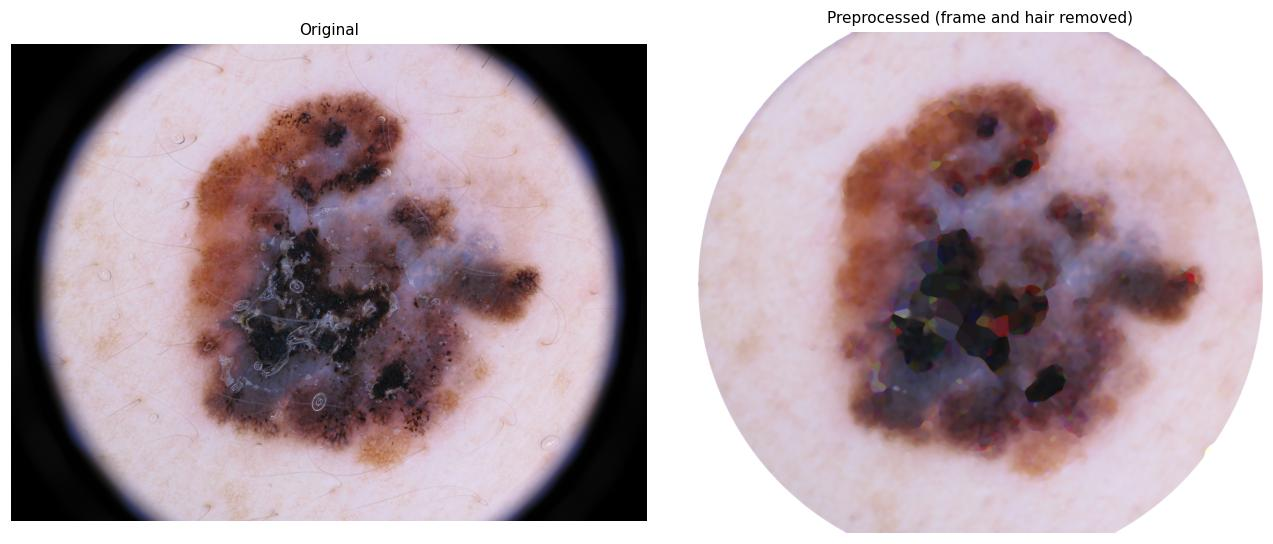
\includegraphics[width=0.9\textwidth]{preprocessing.jpg}
  \caption{Preprocessing. Left: the raw dermoscopic image with its dark frame.
  Right: after frame removal and hair removal. The corners are whitened and the
  image cropped to the dermoscope disc.}
  \label{fig:preprocessing}
\end{figure}

\paragraph{Discussion.} This step proved robust on the majority of standard
images. Simple thresholding can nevertheless show its limits when the frame is
partially reflective or the illumination strongly heterogeneous. Integrating
shading-correction techniques~\cite{cavalcanti}, which model illumination
variation by a quadratic function, would be a natural improvement. For this
project the current method was sufficient.

One consequence of whitening the corners deserves emphasis, because it caused a
real failure later in the pipeline: the whitened area is \emph{synthetic}, not
skin. Any method fitting a global colour model over the whole frame will let
those pixels form a cluster of their own. Section~\ref{sec:lbp} returns to this.

\subsection{Hair removal}

Dermoscopic images often contain hairs crossing the lesion or the surrounding
skin. These artefacts mislead segmentation algorithms, which read them as
contours or as internal lesion structures.

Our approach is based on the reference algorithm DullRazor~\cite{dullrazor},
which detects thin dark structures by morphological closing.

\subsubsection{First approach: naive implementation and its limits}

We first tested a standard implementation using thin linear structuring elements
(one pixel wide) and a high global threshold (250) on the difference image.

\paragraph{Analysis of the failure.} This showed critical limits on images with
thick or low-contrast hairs.

\begin{enumerate}
  \item \textbf{Scale problem.} The structuring element being thinner than some
  hairs, the closing operated \emph{inside} the hair without removing it, making
  detection impossible.
  \item \textbf{Threshold problem.} A threshold of 250 demanded near-maximal
  contrast (black on white). The actual intensity difference between a brown
  hair and skin is often between 20 and 50, so the resulting binary mask was
  mostly empty and no interpolation could take place.
\end{enumerate}

\subsubsection{Second approach: a robust pipeline}
\label{sec:hair-pipeline}

The improved version works as follows:

\begin{enumerate}
  \item \textbf{Multi-directional closing.} Rather than thin lines, we use
  structuring elements $10$ pixels wide and $50$ long, at $0^\circ$, $45^\circ$,
  $90^\circ$ and $135^\circ$, and take the pixelwise maximum of the closings. A
  closing erases any dark structure its element cannot fit inside, so a hair
  thinner than $10$ pixels is erased whatever its orientation.
  \item \textbf{Detection and dilation.} The hair mask is the absolute
  difference between the original and the closed image, thresholded at 40
  instead of 250, since the difference between a brown hair and skin is often
  only 20 to 50. The mask is then dilated by a $20 \times 20$ square to include
  the blurred edges of thick hairs.
  \item \textbf{Interpolation and smoothing.} Masked areas are reconstructed by
  nearest-neighbour grid interpolation from the immediate neighbourhood, and a
  final median filter with a $20 \times 20$ window blends the corrections into
  the surrounding healthy skin.
\end{enumerate}

A coverage test guards the whole stage: the dilated hair mask is eroded by a
disc of radius 12, so that isolated thin detections vanish, and if what
survives covers less than $3\,\%$ of the valid area, the image is returned
untouched. Inpainting a hairless image only blurs the very border the
segmentation is looking for. An earlier version summed the raw intensity
difference here instead of counting pixels, a quantity on a different scale
from the fraction it was compared to; it now counts pixels.

\subsubsection{What the detector actually detects}
\label{sec:hair-limits}

The detector responds to any dark structure narrower than some of its
elements, and the dark, textured interior of a lesion is such a structure.
Five of the twenty images pass the coverage test. Two are genuinely hairy
(\texttt{ISIC\_0000042} and \texttt{ISIC\_0000095}) and one has a few thin
hairs (\texttt{ISIC\_0000146}). The other two (\texttt{ISIC\_0000140} and
\texttt{ISIC\_0000142}) have no visible hair, and on them almost all of the
flagged pixels lie inside the lesion: the stage then inpaints parts of the
lesion itself, which produces the small coloured shards visible in
Figure~\ref{fig:preprocessing}.

The two diagonal elements were added on the belief that the axis-aligned
ones missed diagonal hairs. They do not: every element is 10 pixels wide, so
each of them already erases any thinner hair at any angle. What the diagonals
add is more of the lesion's texture. A detector that separates hair from
lesion texture, for instance by requiring elongation, is left as future work,
and the scores reported here include this weakness.

\section{Segmentation methods}

Having cleaned the artefacts, the critical step is isolating the pigmented
lesion from healthy skin. We implemented and compared three representative
families of algorithms: a histogram-based method (Otsu), a texture-based method
(LBP Clustering) and a region-merging method (SRM).

All three compute on a $256 \times 256$ copy of the image and upscale the
resulting mask. The lesion border is a large-scale structure, so this loses no
useful detail, and it keeps the three methods comparable by giving them the same
amount of information.

\subsection{Method 1: multi-channel Otsu thresholding}
\label{sec:otsu}

\subsubsection{Theoretical principle}

Otsu's method is the classical approach to image binarisation. It assumes the
intensity histogram is bimodal (background and object) and searches for the
threshold $T$ minimising intra-class variance, equivalently maximising the
inter-class variance
\[
\sigma_B^2(T) = \omega_0(T)\,\omega_1(T)\,\bigl[\mu_0(T) - \mu_1(T)\bigr]^2,
\]
where $\omega_0, \omega_1$ are the class probabilities (skin/lesion) and
$\mu_0, \mu_1$ their respective means.

\subsubsection{Multi-channel combination}

The performance of a global threshold depends drastically on the colour channel
used~\cite{garnavi}. A lesion may be invisible in the red channel, where skin and
melanin reflect light similarly, yet strongly contrasted in blue.

Otsu's threshold is therefore computed independently on the red, green and blue
channels, and the three binary masks combined as
\[
M = (M_R \wedge M_G) \vee M_B .
\]
A pixel is lesion when red \emph{and} green agree, or when blue alone is
confident. The asymmetry is deliberate: melanin absorbs short wavelengths
preferentially, so blue carries the strongest melanin contrast and is trusted on
its own, whereas red and green are required to corroborate each other.

The resulting mask has ragged borders. It is therefore used as the initial level
set of a morphological Chan-Vese active contour, run for five iterations, which
relaxes the border onto the actual intensity boundary.

\begin{figure}[H]
  \centering
  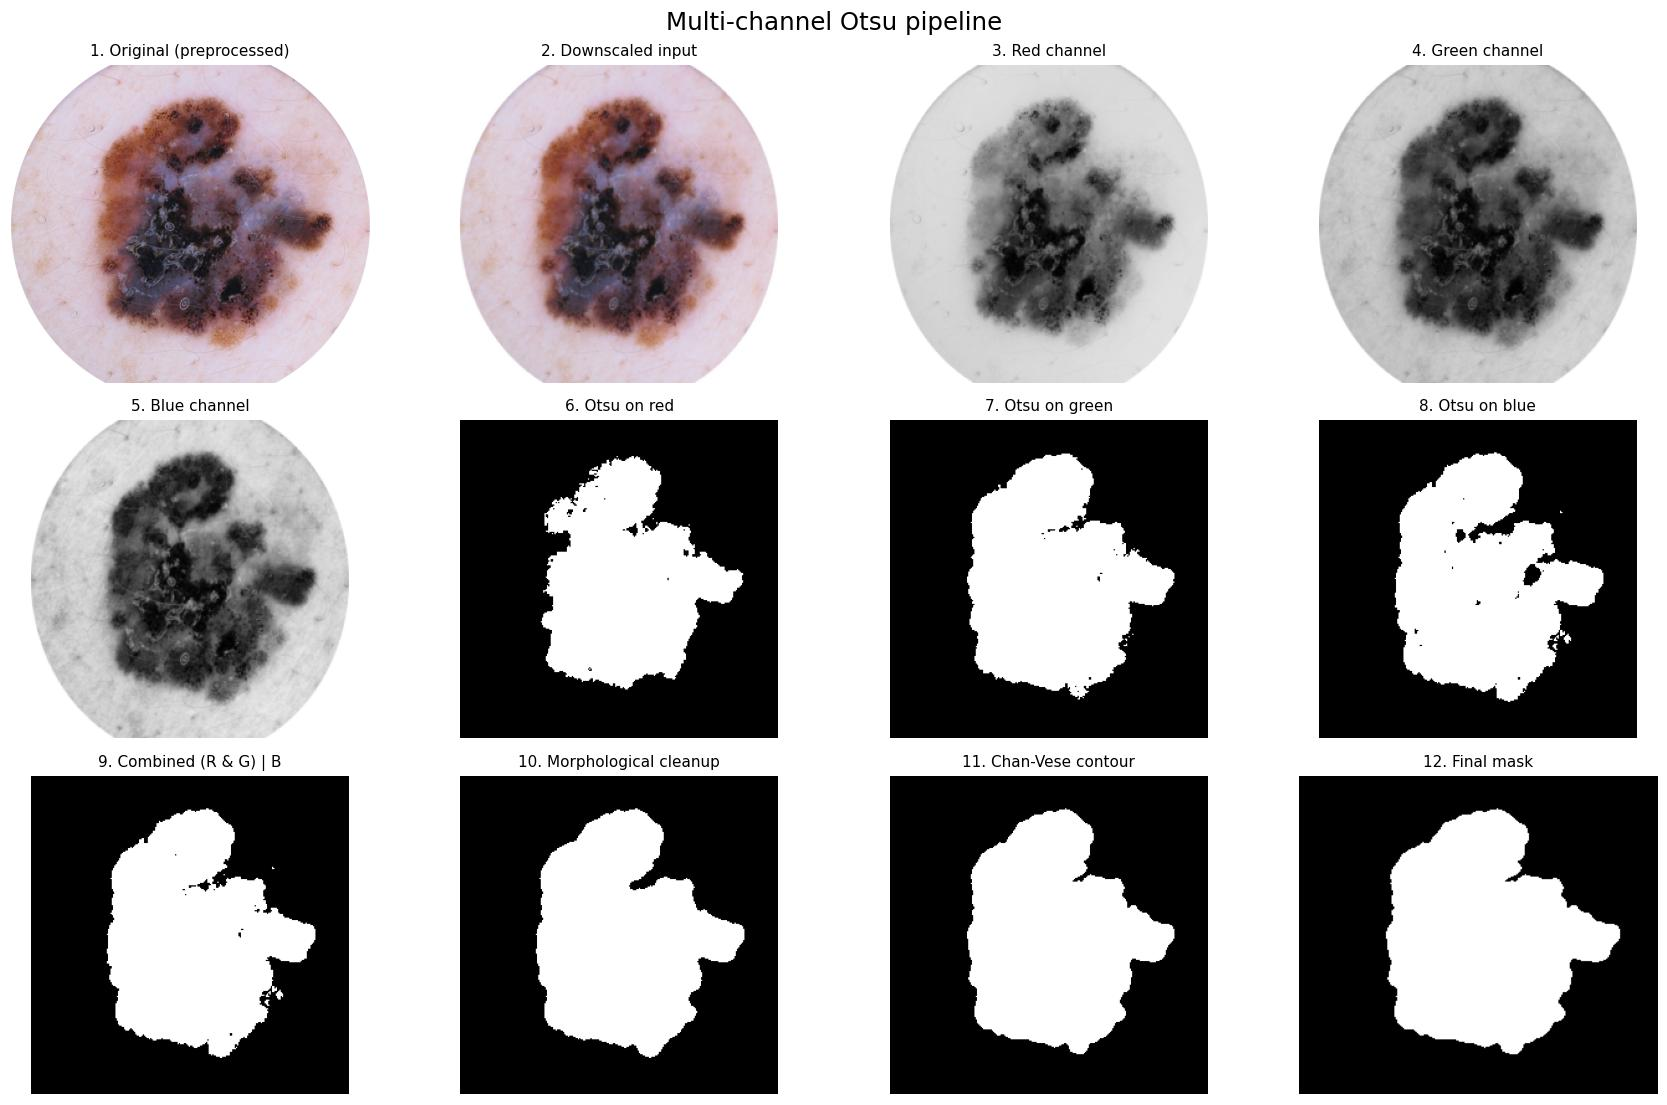
\includegraphics[width=\textwidth]{otsu_pipeline.jpg}
  \caption{The multi-channel Otsu pipeline, stage by stage: the three colour
  channels, their individual Otsu masks, the combination, the morphological
  cleanup and the Chan-Vese refinement.}
  \label{fig:otsu}
\end{figure}

\subsubsection{Observed limitations}

Despite its speed, the method shows intrinsic limits on our dataset. Being
global, it fails when the image presents strong vignetting or cast shadows, the
shadow being segmented as part of the lesion. For early or very pale melanomas
the histogram is not clearly bimodal, and the computed threshold merges the
lesion with the surrounding skin, causing critical under-segmentation.

\subsection{Method 2: LBP Clustering}
\label{sec:lbp}

Simple thresholding fails when the lesion colour is too close to that of the
skin. We therefore implemented a texture-based method following Pereira et
al.~\cite{lbp}, whose founding assumption is that healthy skin has a smooth,
regular texture whereas a lesion has a chaotic one, with its pigment network,
globules and dots.

\subsubsection{Local Binary Patterns and pattern-subset binarisation}

The luminance $Y$ is computed according to ITU-R BT.601,
\[
Y = 0.299\,R + 0.587\,G + 0.114\,B .
\]
For each pixel, the Local Binary Pattern with $P = 8$ neighbours at radius
$R = 1$ encodes the sign of the difference between each neighbour and the
centre, packing the eight bits into a code in $[0, 255]$. The comparison is
strict, matching the paper's $s(u) = \mathbf{1}[u > 0]$.

The key step is the binarisation on a \emph{subset} of patterns. Code $0$ (no
neighbour brighter) and the eight powers of two (exactly one brighter neighbour)
describe locally smooth neighbourhoods; every other code describes texture.
Mapping the smooth subset to $0$ and all others to $1$ yields a texture map
whose ones concentrate inside the lesion.

\subsubsection{Pseudo-RGB construction and the pinkness criterion}

The binary texture map is smoothed by a Gaussian filter ($\sigma = 3$) and
normalised into a continuous field $L \in [0,1]$. The method then builds a
\emph{synthetic} image by stacking
\[
\text{pseudo-RGB} = [\,L,\; Y,\; L\,],
\]
and converts it to CIE L*a*b*, keeping only the chromaticity components
$(a^*, b^*)$. This is the elegant part of the method: a texture quantity and a
luminance quantity are deliberately placed in a colour space so that a
\emph{colorimetric} criterion can separate them.

A $k$-means++ clustering with $k = 2$ partitions the pixels in that $(a^*, b^*)$
plane. Which of the two clusters is the lesion is decided without supervision by
the \emph{pinkness} score
\[
\mathcal{P} = \operatorname{mean}\bigl[\max(a^*, 0) - \min(b^*, 0)\bigr],
\]
the cluster with the higher score being retained. A morphological opening
finishes the mask.

\subsubsection{Interaction with frame removal}
\label{sec:lbp-frame}

Applying the method as published to our cropped images failed completely on
all three framed ones, with a raw Dice score of exactly zero. The cause is the interaction
announced in Section~\ref{sec:frame-removal}: frame removal whitens the corners, and a white pixel
has $L = 0$ texture with $Y = 255$, so in the pseudo-RGB it becomes
\emph{pure green}, an extreme point in the $(a^*, b^*)$ plane. Those synthetic
pixels captured one of the two clusters outright, and $k$-means separated disc
from corners instead of lesion from skin.

Restricting the clustering to the valid disc area resolves it, and the three
failing images rose from $0.000$ to $0.708$, $0.895$ and $0.906$. The lesson generalises
beyond this project: a preprocessing step that fabricates pixel values must
publish which pixels it fabricated.

\begin{figure}[H]
  \centering
  
\includegraphics[width=\textwidth]{lbp_pipeline.jpg}
  \caption{The LBP Clustering pipeline: luminance, LBP codes, the binarised
  texture patterns, the smoothed field $L$, the pseudo-RGB $[L, Y, L]$, its
  chromaticity components, the $k$-means clusters and the cluster selected by
  the pinkness criterion.}
  \label{fig:lbp}
\end{figure}

\subsection{Method 3: Statistical Region Merging}

SRM~\cite{celebi} is a region-growing technique. Every pixel starts as its own
region, and adjacent regions are merged iteratively when they are statistically
similar.

\subsubsection{The merging predicate}
\label{sec:srm-predicate}

Pairs of 4-connected neighbouring pixels are sorted by increasing absolute
intensity difference and visited in that order, so the most obviously similar
neighbours merge first. Two regions $R_1$ and $R_2$ are merged when
\[
\bigl(\overline{R_1} - \overline{R_2}\bigr)^2 < b(R_1) + b(R_2),
\qquad
b(R) = \frac{g^2}{2Q\,|R|}\Bigl(\ln(1 + |R|) + 2\ln(6n)\Bigr),
\]
where $\overline{R}$ is the region mean, $|R|$ its size, $n$ the pixel count and
$g = 1$ for intensities in $[0,1]$. The bound tightens as regions grow: early
merges are cheap, late merges must be well supported. The scale parameter $Q$
controls permissiveness, a smaller $Q$ yielding fewer, larger regions. Regions
are maintained in a union-find structure with path compression and union by
rank.

The implementation follows the algorithm directly rather than calling a library,
and the smoothing is applied to the grayscale image, not to the colour image: a
scalar Gaussian $\sigma$ on an $(H, W, 3)$ array also blurs \emph{across} the
channel axis, mixing red into blue, and it measurably degraded the region
scoring before it was found. The Felzenszwalb backend, kept for comparison, had
the same mistake; it now smooths each colour channel separately.

\subsubsection{From regions to a lesion}

SRM produces an over-segmentation, not a lesion. Each region is scored on three
criteria, combined as $0.5\,c + 0.3\,z + 0.4\,s$:

\begin{itemize}
  \item \textbf{Contrast} $c$ against skin. The skin reference is the 70th
  percentile of a one-pixel band along the image border, following the
  observation of Zortea et al.~\cite{zortea} that this band is mostly healthy
  skin. That holds on unframed images; on framed ones it does not
  (Section~\ref{sec:frame-blind-spot}). The blue channel is used, for the
  melanin-absorption reason
  given in Section~\ref{sec:otsu}.
  \item \textbf{Centrality} $z$, a prior that the lesion lies near the centre.
  \item \textbf{Saturation} $s$, the HSV saturation above the skin median, which
  detects erythematous areas that are bright but pathological.
\end{itemize}

Polychrome lesions, a dark core with a brown periphery, are split by the
over-segmentation, and keeping only the best region under-estimates the area. We
therefore merge the winning region with every region scoring above 60\,\% of the
maximum \emph{and} genuinely darker or more saturated than skin. The second
condition prevents the mask from creeping into shaded skin.

\begin{figure}[H]
  \centering
  
\includegraphics[width=\textwidth]{srm_pipeline.jpg}
  \caption{The SRM pipeline: smoothing, the union-find over-segmentation, the
  blue and saturation channels driving the scoring, the resulting score map, the
  selected regions and the final mask.}
  \label{fig:srm}
\end{figure}

\subsection{Otsu and SRM's blind spot to the frame corners}
\label{sec:frame-blind-spot}

Section~\ref{sec:lbp-frame} covers why LBP's clustering has to ignore the
whitened frame corners left by frame removal. Otsu and SRM have the same
vulnerability. Otsu's per-channel threshold reads the corners as an
artificially bright cluster. SRM reads its skin reference off a one-pixel band
along the image border, and on a framed image, whose crop is the disc's
bounding box, most of that band runs through the whitened corners
($65$--$72\,\%$ of it on this dataset's three framed images), so the "skin"
reference is largely the white of the corners.

Otsu's threshold is now computed on the valid pixels only. This does not raise
Dice: on the three framed images it lowers it very slightly, by $0.001$ to
$0.006$. It is kept because a threshold meant to separate lesion from skin
should be computed on lesion and skin only.

The same change to SRM's reference lowers its Dice on all three framed
images, by $0.07$ to $0.21$, because the hand-tuned weights and thresholds
that judge a region's score were calibrated against the biased reference.
Fixing it properly means retuning those weights, which is out of scope here.
\texttt{region\_merging.segment} keeps the corrected reference as an opt-in
parameter, tested in isolation, and the benchmark does not enable it.

\subsection{Post-processing: the smart convex hull}

Using a convex hull to smooth borders is common practice but risky. On some
images a small residual artefact in a corner produced an aberrant triangular
mask spanning the whole image.

Before computing the hull, our \texttt{smart\_convex\_hull} filter analyses the
connected components of the mask. It always keeps the largest, and keeps a
satellite component only if it lies close to it, within a quarter of the
image diagonal (Section~\ref{sec:four-guards} explains both choices). Distant
specks of noise are discarded, so the convex shape stays meaningful.

The same post-processing (clipping to the valid area, hole filling and this
hull) is applied identically to all three methods, so that the comparison
isolates the segmentation itself.

\subsubsection{Post-processing guards that were not doing what they claimed}
\label{sec:four-guards}

An audit of this stage found its heuristics measuring the wrong quantity,
silently, in four places. None of them raised an error. All four are fixed or
removed in the version of the code this report describes.

\paragraph{\texttt{clean\_mask} clipped to a guessed disc, not the real one.}
The dermoscope disc is known exactly: frame removal (Section~\ref{sec:frame-removal}) already
computes it and returns it as a valid-area mask. \texttt{clean\_mask} did not
use it. Instead, on \emph{every} image, it inscribed a circle in the array's
own bounding box, regardless of whether that image had a frame at all.
Seventeen of the twenty images in this dataset have none, so on those the
guessed circle is fiction, and every lesion pixel that happened to fall
outside it was deleted before scoring. On \texttt{ISIC\_0000049}, whose lesion
reaches toward a corner, applying the old guessed-disc crop to the ground
truth itself erases $20.4\,\%$ of its area, a loss with nothing to do with
segmentation quality, incurred before any method is even compared to the
truth. The fix threads the real valid-area mask from preprocessing through to
\texttt{clean\_mask}, so the crop matches the disc that was actually removed,
or clips nothing at all on an unframed image.

\paragraph{An inversion guard that could only do harm.} \texttt{clean\_mask}
also flipped any mask covering more than $60\,\%$ of the valid area, on the
theory that a segmenter covering that much had selected skin instead of
lesion. On this dataset no segmenter output covers more than about $45\,\%$ of
the valid area, while two real lesions (\texttt{ISIC\_0000030} and
\texttt{ISIC\_0000049}) cover more than $60\,\%$. The guard therefore never
rescued anything, and would have turned a perfect segmentation of those two
lesions into its complement. It was removed, and a unit test now checks that
a large lesion comes through post-processing intact.

\paragraph{The hull's satellite reach grew with the lesion, past the image
itself.} A satellite blob was kept if it lay within $2.5$ lesion radii of the
main component, a reach that scales with the lesion. On a large lesion that
reach can exceed the image: on \texttt{ISIC\_0000145}, it worked out to
$1376$\,px, while the single farthest point in the image (a corner) sits at
only $1327$\,px. Every pixel therefore counted as "close enough", and the
filter had nothing left to reject on that image, defeating the purpose stated
at the top of this subsection. The fix measures the reach as a fraction of the
image diagonal ($0.25\times$) instead of the lesion's own radius. Across this
dataset the farthest corner sits at $51$–$58\,\%$ of the diagonal regardless of
lesion size, so this reach stays below that on every image while remaining
generous enough to keep a genuinely nearby fragment.

\paragraph{A satellite kept for being large had no distance limit at all.}
The reach fixed above applied only to a satellite kept for being
\emph{close}; one kept for being \emph{large} (more than $3\,\%$ of the main
component's area) was exempt from any distance check, on the reasoning that a
sizeable second lobe of the same lesion should count regardless of where it
sits. That reasoning fails in practice: on \texttt{ISIC\_0000095}, the LBP
method's texture criterion also flags patches of scaly skin scattered across
the image, far from the lesion, and the old rule glued the large ones into the
hull. The buggy hull scores just $0.189$ Dice on this image, and the fix
(distance alone) recovers it to $0.694$. Being large gave a region no more
claim to belonging to the lesion than being small, so every satellite is now
judged by the same reach, however large it is.

\paragraph{Why these went unnoticed.} All four are silent by construction: a
guard that never fires looks identical, in code and in a spot check, to a
guard that never needed to fire. They surfaced only by asking, of each
threshold, what quantity it was actually being compared against on this
dataset's real image shapes and real segmenter outputs.

\section{Results and discussion}
\label{sec:results}

\subsection{Quantitative analysis}

Each predicted mask is compared to the expert ground truth by the Dice
coefficient. Table~\ref{tab:overall} gives the means over the \nimages{} images.

\paragraph{Scoring a cropped image against its ground truth.} Frame removal
crops the three framed images to the disc's bounding box, so their masks are
narrower than the ground truth. An earlier version of the pipeline resized the
full-size ground truth to the cropped shape, squeezing it sideways instead of
cutting the same columns off: prediction and truth no longer described the
same pixels, and a \emph{perfect} segmentation of those images scored only
$0.915$ to $0.965$. The ground truth is now cropped with the exact box frame
removal uses, and a unit test checks that a perfect mask on a framed image
scores $1$. The fix lowered every method's raw score on all three framed
images, by up to $0.066$ (the stretched truth happened to flatter them), and
each method's mean raw Dice by $0.002$ to $0.006$. The ranking is unchanged.
Every number in this report is measured after the fix.

\begin{table}[H]
  \centering
  \overalltable
  \caption{Mean Dice coefficient per method.}
  \label{tab:overall}
\end{table}

Two trends stand out.

\paragraph{The convex hull helps all three methods by a similar margin.} It
raises the mean Dice of Otsu, LBP and SRM alike by roughly $0.049$ to
$0.060$. It is not a uniform improvement: on three images
(\texttt{ISIC\_0000001}, \texttt{ISIC\_0000145} and \texttt{ISIC\_0000080}) it
costs LBP between $0.012$ and $0.027$ Dice, because the raw mask was already
close to the lesion's true shape and the added convexity is pure loss there.
Convexity is an \emph{assumption} about lesion shape, and it does not hold
uniformly.

\paragraph{Texture gives the best raw masks, by a narrow margin.} LBP
Clustering produces the best masks before post-processing, ahead of Otsu and
SRM, and with the hull applied it is also the best method overall. On twenty
images these gaps are small, so the ranking is indicative rather than
definitive.

\subsection{Melanoma versus nevus}

\begin{table}[H]
  \centering
  \categorytable
  \caption{Mean Dice coefficient per method and per diagnosis.}
  \label{tab:category}
\end{table}

Melanomas score lower than nevi on average in five of the six columns, which
is the clinically expected direction: irregular, poorly defined borders are
precisely what characterises melanoma. With ten images per class, however,
none of these gaps is statistically significant (two-sided Mann--Whitney test,
$p > 0.4$ in every column), and LBP's raw masks score the same on both
diagnoses ($0.842$ against $0.841$). This dataset cannot establish that
melanomas are harder to segment.

\begin{figure}[H]
  \centering
  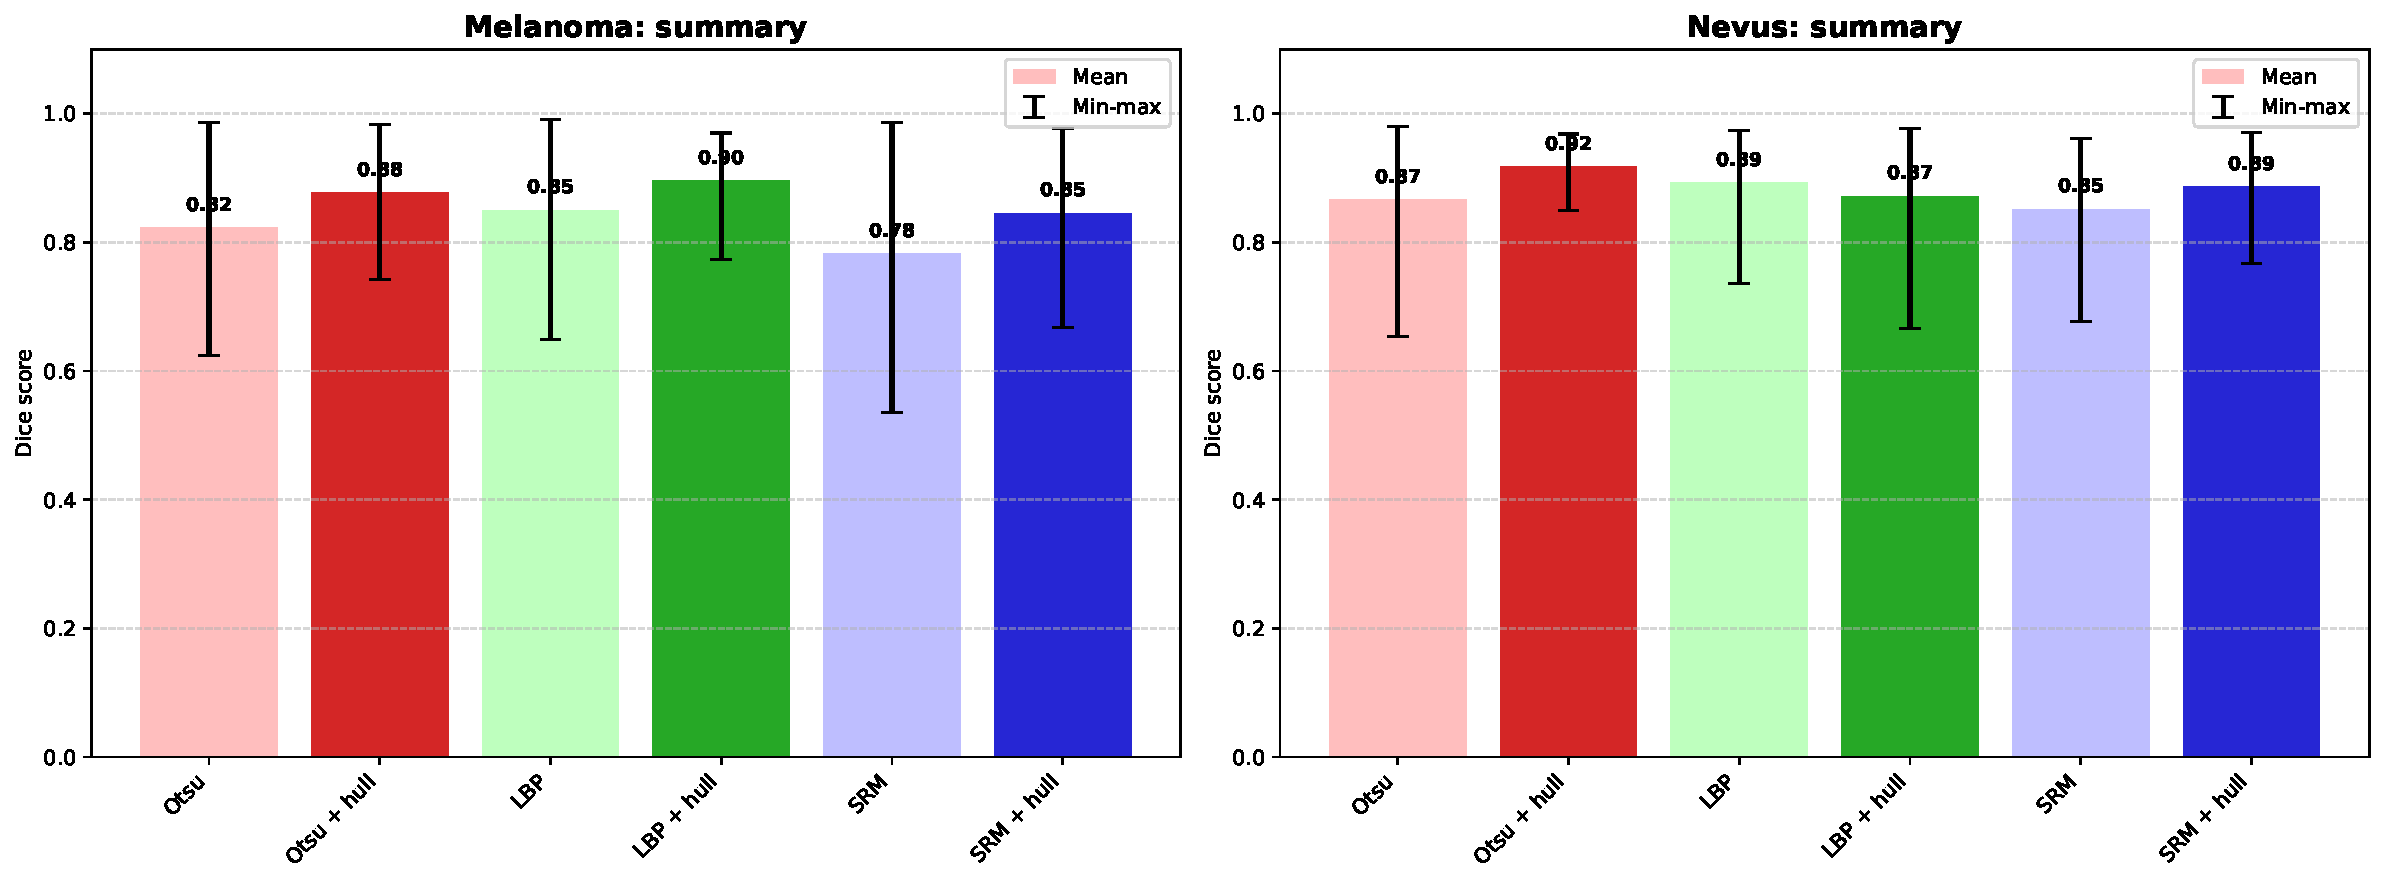
\includegraphics[width=\textwidth]{dice_summary.pdf}
  \caption{Mean Dice per method with min--max whiskers, melanoma (left) and
  nevus (right). SRM's spread is much wider on melanomas, down to $0.47$ on
  \texttt{ISIC\_0000049}; Otsu's is similar on both, and LBP's is wider on nevi,
  where \texttt{ISIC\_0000095} pulls it down.}
  \label{fig:summary}
\end{figure}

\subsection{Failure analysis}

The per-image scores in Table~\ref{tab:perimage} make the failure modes
explicit.

Two images drag every method's raw mask below $0.70$. ISIC\_0000024 is a
low-contrast lesion where neither an intensity nor a texture cue separates
lesion from skin cleanly. ISIC\_0000049 is also the largest lesion in the set,
and every method captures only part of it; whether its contrast or its size
is to blame (the centrality prior and the border-sampled skin reference both
assume a lesion well inside the image) is not established here. The convex
hull recovers these two unevenly, lifting LBP above its own average on
ISIC\_0000024. These are the cases where a learned model, given enough
annotated data, would most likely do better.

\begin{table}[H]
  \centering
  \small
  \perimagetable
  \caption{Dice coefficient per image and per method.}
  \label{tab:perimage}
\end{table}

\begin{figure}[H]
  \centering
  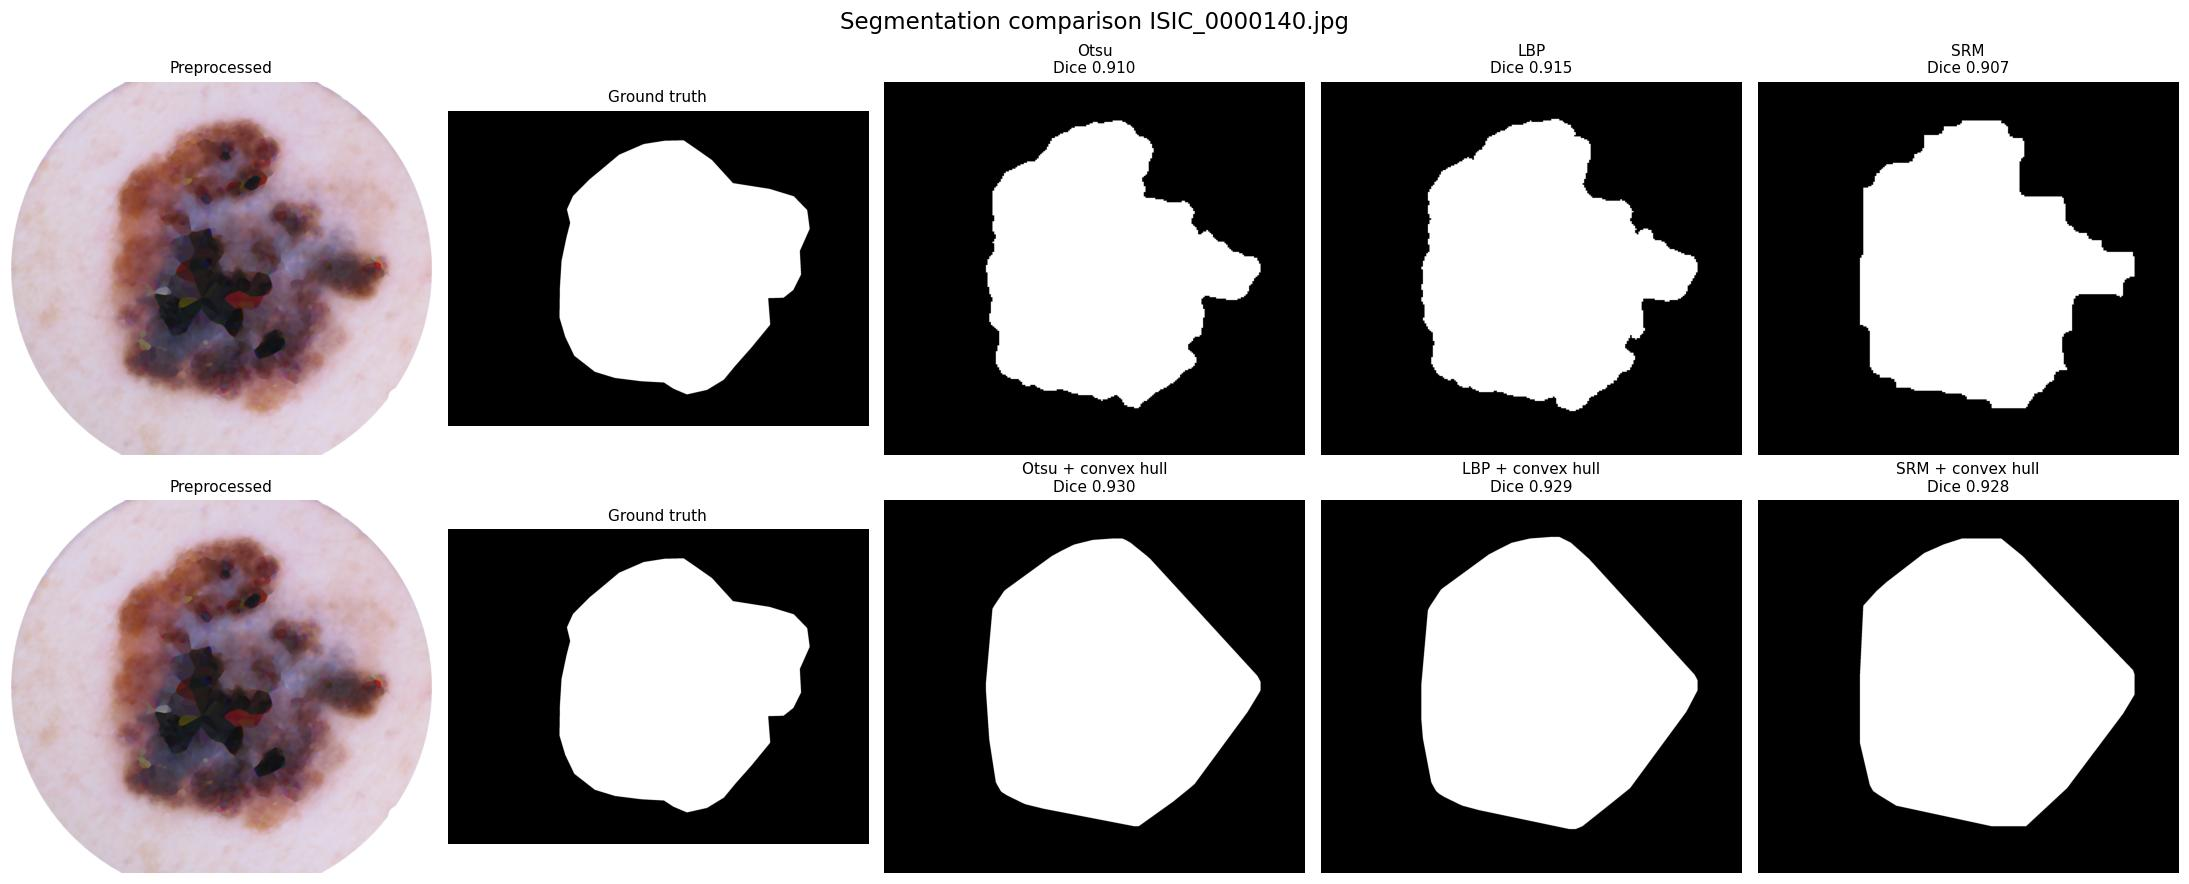
\includegraphics[width=\textwidth]{method_comparison.jpg}
  \caption{The three methods against the ground truth on one melanoma, with and
  without the convex hull.}
  \label{fig:comparison}
\end{figure}

\subsection{Limitations}

These numbers should be read with their limits in mind.

\begin{itemize}
  \item \textbf{Twenty images is a demonstration, not an evaluation.} No
  confidence interval computed on this sample would be meaningful.
  \item \textbf{Parameters were tuned on these same images.} There is no
  held-out set, so the reported scores are optimistic.
  \item \textbf{The hair detector also detects lesion texture.} On two
  hairless images it inpaints parts of the lesion itself
  (Section~\ref{sec:hair-limits}), and the scores include that weakness.
  \item \textbf{A single ground truth per image.} Expert delineations vary
  between dermatologists, and the Dice ceiling attainable is bounded by that
  variability, which we cannot measure with one annotation.
\end{itemize}

\section*{Conclusion}

We implemented a complete skin-lesion segmentation pipeline using classical
computer vision only, from artefact removal through to quantitative evaluation,
and compared three methods reimplemented from their source publications.

The outcome contradicts our initial expectation. We had assumed the most
sophisticated method, region merging, would dominate; it does not. The
texture-based LBP Clustering gives the best raw masks, and the simplest method,
multi-channel Otsu, is highly competitive once the convex hull is applied.
Algorithmic sophistication did not translate into accuracy on this dataset.

Two findings proved more instructive than the ranking itself. First, the
interaction between frame removal and the LBP clustering, where a preprocessing
step that fabricates pixel values silently destroyed a method that fits a global
colour model, a class of bug invisible in the mean and obvious in the pipeline
figures. Second, the cost of smoothing a colour image with a scalar Gaussian,
which blurs across the channel axis and quietly corrupted the region scoring.
Both were found by inspecting intermediate stages, which is exactly the
affordance that a classical pipeline offers and a network does not.

The natural continuations are shading correction~\cite{cavalcanti} to handle
heterogeneous illumination, evaluation on a larger ISIC subset with a held-out
parameter set, and using these masks as the input to the feature-extraction
stage of a full CAD system.

\begin{thebibliography}{9}

\bibitem{dullrazor}
T.~Lee, V.~Ng, R.~Gallagher, A.~Coldman and D.~McLean.
\newblock DullRazor: A software approach to hair removal from images.
\newblock \emph{Computers in Biology and Medicine}, 27(6):533--543, 1997.

\bibitem{cavalcanti}
P.~G.~Cavalcanti, J.~Scharcanski and C.~B.~O.~Lopes.
\newblock Shading Attenuation in Human Skin Color Images.
\newblock \emph{ISVC 2010}, LNCS 6453:190--198, 2010.

\bibitem{lbp}
P.~M.~M.~Pereira, R.~Fonseca-Pinto, R.~P.~Paiva, P.~A.~A.~Assunção,
L.~M.~N.~Tavora, L.~A.~Thomaz and S.~M.~M.~Faria.
\newblock Dermoscopic skin lesion image segmentation based on Local Binary
Pattern Clustering: Comparative study.
\newblock \emph{Biomedical Signal Processing and Control}, 59:101924, 2020.

\bibitem{celebi}
M.~E.~Celebi et al.
\newblock Border detection in dermoscopy images using statistical region
merging.
\newblock \emph{Skin Research and Technology}, 14(3):347--353, 2008.

\bibitem{garnavi}
R.~Garnavi, M.~Aldeen, M.~E.~Celebi, A.~Bhuiyan, C.~Dolianitis and G.~Varigos.
\newblock Skin Lesion Segmentation Using Color Channel Optimization and
Clustering-based Histogram Thresholding.
\newblock \emph{International Journal of Biomedical and Biological
Engineering}, 3(12), 2009.

\bibitem{zortea}
M.~Zortea, E.~Flores and J.~Scharcanski.
\newblock A simple weighted thresholding method for the segmentation of
pigmented skin lesions in macroscopic images.
\newblock \emph{Pattern Recognition}, 64:92--104, 2017.

\end{thebibliography}

\end{document}
